% declara a section
\section{Introduç\~ao ao livro.} % declarando uma section.
Esse livro tem como objetivo armazenar todo o conhecimento do grupo ROBOTA,
ajudando novos membros e colaborando com o ambiente acadêmico.

%declara a subsection
\subsection{Sobre THE BIG BOOK OF ROBOTA.}	% declarando uma subsection.
Esse livro teve inicio no fatídico dia (04/11/2013) para maior organizaç\~ao do grupo,
unir toda a documentaç\~ao e evitar o retrabalho.

Este livro esta separado em 5 capítulos:

% enumerando alguns tópicos
\begin{enumerate}
\item Introdução
\item Software
\item Hardware
\item Mecânica
\item Gerencial
\end{enumerate}

Cada capitulo possui uma pasta e cada pasta possui outra para as seções, como mostrado na fugira \ref{estrutura}.

% adicionando uma figura
% o caminho da figura tem que ser des da raiz.

\begin{center}
\center
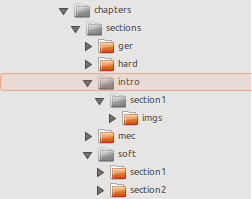
\includegraphics[width=6cm]{./include/chapters/sections/intro/section1/imgs/estrutura.png}

\section{Estrura de pastas.}
\label{estrutura}
\end{center}

Essa estrutura pode ser detalhada da seguinte forma:\\										% serve para quebrar a linha
A pasta raiz do THE BIG BOOK OF ROBOTA contem a pasta include, que por sue vez contem a pasta chapters,
cada aquivo tex dentro desta pasta possui os caminhos para sections.\\

Assim, caso algu\'em queira adicionar mais um arquivo ao grandioso e inigualável THE BIG BOOK OF ROBOTA, 
\'e s\'o seguir o que \'e dito na proxima subsection (~\ref{subsec:adicionandosuacontribuicao}).		% referenciando o label

\subsection{Adicionando sua contribuição.} ~\label{subsec:adicionandosuacontribuicao}			% adicionando um label para ser referenciado

Bem, vamos l\'a, primeiramente podes utilizar essa pr\'opria section como exemplo, ela est\'a em:\\
root/include/chapters/sections/intro/section1\\													
Podendo encontrar o arquivo tex, esse seria como um ambiente de trabalho, onde existe o seu tex
e uma pasta para imagens da sua section. \\
Após criar seu tex, vamos adicionar ele ao nosso livro.\\
Primeiramente vá até: 
root/include/chapters/\\
Entre no tex do capitulo que gostaria adicionar seu tex, agora é só adicionar a seguinte linha ao documento:\\
input\{./include/chapters/sections/XXX/sectionX/section.tex\}\\
Onde XXX seria o nome da pasta do capitulo e X o numero da section.\\
Simplificando seria os seguintes paços:\\

% enumerando paços
\begin{enumerate}
\item Crie seu .tex 
\item Dentro da pasta sections, entre na pasta do chapter que gostaria de adicionar e crie uma pasta sectionX para adicionar seu .tex 
\item Ap\'os adicionar seu arquivo, inclua o caminho dele dentro da arquivo .tex como exemplificado dentro de intro.tex
\item N\~ao esqueça de quando for compilar, sempre compilar o arquivo main.tex, não o arquivo .tex da section !!
\end{enumerate}

\author{Patrick J.P}		% adicionando um autor

